\documentclass[10pt,twoside]{./template/StyleUBI}

\usepackage{./template/FormattingUBI}

\usepackage{array,verbatim}
\setmainfont{Trebuchet MS}

%%Comentar a linha seguinte se escrever a tese em inglês
\portugues

%%Para índice remissivo
\makeindex

\thesistitle{Título da Tese}
%\thesissubtitle{An comprehensive approach}
\thesisauthors{Nome do autor}
\thesistype{PhD Thesis Proposal}
\thesislocalanddate{Covilhã, May of 2016.}
\thesissupervisors{
	Supervisor: Prof. Doutor Nome\\
	%Orientador: Prof. PhD Nome\\
	Co-supervisor: Prof. Doutor Nome\\
}
\thesiscourse{Engenharia Informática}

%%Escolher tipo de letra a usar:
%\usepackage{lmodern} 	%Latin modern
%\usepackage{palatino} 	%Palatino
%\usepackage{times} 	%Times
%\renewcommand{\rmdefault}{trebuchet} 	%Trebuchet (caso esteja instalado)


%%O comando seguinte insere o nome da tese no cabeçalho das páginas (comentar se não for pretendido)
%(Pode ser um título abreviado)
\cabecalho{\thesistitlestr}

\begin{document}
%%Dedicatória (se não desejar incluír dedicatório, todo o comando deve ser apagado)
%Isto vale para todas as seções abaixo.
\thesisdedication{
    %Se desejar colocar o conteúdo em um ficheiro tex separado,
    %ele pode ser incluído usando o comando \input{Nome do ficheiro criado}.
    %Isto resulta para todas as seções abaixo.
	Inserir dedicatória (opcional)
}

%%Agradecimentos 
\thesisthanks{
	Agradecer a quem de direito (opcional)
}

%%Prefácio
\thesisforewords{
	Prefácio (Opcional)
}

%%Resumo+palavras-chave (em português)
\thesisresumo{
	Resumo do trabalho
}
{Suas, palavras, chaves, separadas, por, vírgula} 	


%%Resumo alargado (em português)
\thesisresumoalargado{
	Unicamente para teses em língua estrangeira
} 	

%%abstract+keywords
\thesisabstract{
	Abstract in English
}
{Your, key, words, separated, by, comma}	


\tableofcontents %Índice
\listoffigures   %Lista de figuras
\listoftables    %Lista de tabelas

%Lista de Algoritmos (algorithms list)
\newpage
\phantomsection \label{listofalgs}
\addcontentsline{toc}{chapter\label{listofalgs}}{List of Algorithms}
\listofalgorithms
\cleardoublepage


%%Abreviaturas
\phantomsection \label{listofabbreviations}
\addcontentsline{toc}{chapter\label{listofabbreviations}}{List of Abbreviations}
%%Abreviaturas
\newpage
\section*{\titulos{Lista de Acrónimos}}
\vspace{0.5cm}
  \begin{tabularx}{\linewidth}{c p{0.5cm} Y}
 	UBI & & Universidade da Beira Interior\cr
 	MPSOCD & & Multi-objective Particle Swarm Optimization Crowding Distance
 	\end{tabularx}
 \cleardoublepage


\mainmatter

%% Os capitulos são inseridos a partir daqui 
\chapter{Introdução}
\label{chap:int}

%% Para fazer um mini indice do capitulo abrir o ficheiro ``formatacaoUBI.tex" e procurar ''%% O código seguinte permite gerar um mini indice de capitulo (não referido no despacho reitoral)''
%\minitoc




\section{Objectivos}
Este documento pretende servir como modelo\index{modelo} para teses a apresentar na Universidade da Beira Interior (UBI). Para mais informações sobre o {\LaTeX} pode consultar \cite{short} ou \cite{eprojects}.

\section{Secção 2}
\label{sec2}
Lorem ipsum dolor sit amet, consectetur adipiscing elit. Praesent at magna viverra neque bibendum pellentesque. Morbi ullamcorper auctor turpis vitae mollis. Fusce elementum mauris eu magna tristique vel aliquet erat iaculis. Donec sed augue mi. Aenean commodo lorem ac nulla iaculis rhoncus. Mauris facilisis, ante in molestie bibendum, lorem augue vehicula metus, ac auctor turpis quam nec purus. Nam malesuada accumsan neque, quis vulputate nibh dapibus vitae. Vestibulum eu arcu ut est posuere malesuada. Donec aliquet, mauris vel viverra bibendum, risus sem fringilla orci, placerat laoreet felis velit ac justo. Mauris sit amet sollicitudin magna. Sed commodo enim sed nibh consectetur cursus. Duis turpis lacus, semper non facilisis eu, semper eu lacus. Donec vel urna urna, eget gravida magna.

Donec purus ipsum, tincidunt sit amet sagittis varius, sollicitudin ac ipsum. Phasellus quam tortor, volutpat nec interdum a, tristique sed turpis. Aenean fringilla, libero in pretium rhoncus, augue nisi sodales libero, at varius quam ipsum feugiat quam. Vestibulum pharetra pellentesque justo, a scelerisque justo varius ultrices. Nam libero augue, ultricies elementum dignissim nec, tincidunt id mi. Fusce ac ligula nibh, vel molestie metus. 

\section{Secção 3}
\label{sec3}
Aliquam et sapien at augue tempus congue in ac justo. Donec vehicula tempor mi venenatis dictum. In magna mauris, varius vel sollicitudin ac, lobortis et nunc. Suspendisse nec ultrices leo. Proin vehicula imperdiet neque vitae aliquam. Fusce tincidunt mauris sit amet nulla iaculis ac vulputate augue ornare. Praesent quam eros, suscipit ut pulvinar tristique, dapibus vel turpis. Proin commodo pharetra nisl vitae cursus. Cum sociis natoque penatibus et magnis dis parturient montes, nascetur ridiculus mus. Integer eu metus in turpis lobortis blandit. Vivamus euismod rutrum molestie. Morbi luctus orci tempus enim vestibulum facilisis. Etiam dapibus quam id lorem convallis scelerisque. Fusce tristique enim nec ipsum lacinia pretium.

\subsection{Subsecção}

Nam placerat ullamcorper ante non venenatis. Phasellus et ipsum at lorem rhoncus euismod. Phasellus in risus elit, sed mollis dolor. Aenean non ligula ut metus porta laoreet. Duis mi quam, sollicitudin non posuere eu, facilisis vestibulum purus. Cras eget odio et diam imperdiet consectetur eu vel libero. Cras in dapibus felis. Praesent sed nunc neque. Donec lobortis venenatis pretium. Praesent quis lorem ipsum, id mattis ante. 


\chapter{Exemplos}
\label{chap:ex}
Neste \textbf{capítulo} exemplifica-se como inserir alguns ambientes (enumeração, tabela, figura).

\begin{enumerate}
	\item Resistência\index{Resistência} -- É um elemento passivo que dissipa energia sob a forma térmica;
	\item Condensador\index{Condensador} -- É um elemento que armazena energia num campo eléctrico.
\end{enumerate}

A tabela \ref{tab:001} contém o código de cores das resistências\footnote{Apenas código para primeira e segunda cor. Não inclui tolerância nem factor multiplicativo. Apenas código para primeira e segunda cor. Não inclui tolerância nem factor multiplicativo. Apenas código para primeira e segunda cor. Não inclui tolerância nem factor multiplicativo}.

\begin{table}[h!]
\caption{Correspondência entre as cores das riscas das resistências e o seu valor óhmico.}
	\centering
		\begin{tabular}{|c|c|}
		\hline
			\textbf{Cor} & \textbf{Valor} \cr
			\hline
			Preto & 0 \cr
			\hline
			Castanho & 1 \cr
			\hline
			Vermelho & 2 \cr
			\hline
			Laranja & 3 \cr
			\hline
			Amarelo & 4 \cr
			\hline
			Verde & 5 \cr
			\hline
			Azul & 6 \cr
			\hline
			Violeta & 7 \cr
			\hline
			Cinzento & 8 \cr
			\hline
			Branco & 9 \cr
			\hline
		\end{tabular}
	\label{tab:001}
\end{table}

Considere-se o circuito da figura \ref{fig:ohm}.

\begin{figure}[h]
	\centering
		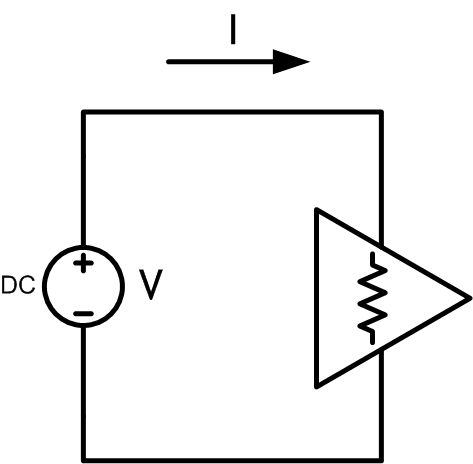
\includegraphics[height=3cm]{leiOhm}
	\caption{Circuito básico com uma fonte de tensão contínua (V) e uma resistência atravessada por uma corrente I.}
	\label{fig:ohm}
\end{figure}

Pode-se calcular a corrente que circula na resistência através da equação \ref{for:ohm}, denominada de Lei de Ohm\index{Lei de Ohm}.

\begin{equation}\label{for:ohm}
	I=\frac{V}{R}
\end{equation}

O texto pode vir em \textbf{negrito} ou em \textit{itálico} ou \textbf{\textit{ambos}}.

O algoritmo \ref{alg1} serve de base para o nosso sistema de controlo do semáforo da igreja.
\begin{algorithm}
\caption{Pseudocódigo para o semáforo}
\label{alg1}
\begin{algorithmic}[1]
\STATE Início
\FOR{todas as luzes}
\IF{sem corrente}
\STATE informar de avaria
\ELSE
\STATE luz ok\ENDIF \ENDFOR
\LOOP
\STATE accionar verde no semáforo principal
\STATE aguardar por sinal dos sensores de posição
\IF{carro no sensor}
\STATE mudar para vermelho semáforo principal
\ENDIF
\ENDLOOP
\STATE \textbf{until} interruptor de manutenção activado
\end{algorithmic}
\end{algorithm}






%% Fim da inserção dos capitulos

%Bibliografia (bibliography)
%Primeiro parâmetro é o estilo e o segundo o arquivo bib
\thesisbibliography{./template/BibliographyStyle}{bibliografia}
%\thesisbibliography{./template/IEEEtran}{references}

%%Anexos
\appendix{
	\chapter{Anexos}
\label{chap:anexos}

\section{Datasheets dos componentes utilizados}


}

%%Glossário
\thesisglossary{
	\begin{tabularx}{\linewidth}{l p{0.5cm} Y}
	\LaTeX & & Conjunto de macros para o processador de textos \TeX, utilizado amplamente para a produção de textos matemáticos e científicos devido à sua alta qualidade tipográfica.\cr
	\end{tabularx}
}

%%Inserir índice remissivo
\printindex

\end{document}
